\documentclass[a4paper,11pt]{scrartcl}
\usepackage{releasenotes}
\usepackage{tabularx}
\usepackage{booktabs}
\usepackage{enumitem}
\usepackage{hyperref}
\usepackage{graphicx}
\usepackage{subcaption}
\usepackage{float}
\graphicspath{{./UI/}}

\title{User Manual\\Kaiju Academy}
\author{Group A2}
\date{\today}

\begin{document}

\maketitle

\section*{User Manual}
\addcontentsline{toc}{section}{User Manual}

\tableofcontents
\newpage

\section{Introduction}

Kaiju Academy is a web-based e-learning platform for programming education, supporting interactive code assessments, course management, and user progress tracking. This manual guides students and educators in using the system’s main features.

\section{System Requirements}
To ensure smooth and reliable access to Kaiju Academy’s features, users must meet the following requirements:
\subsection{Browser}
Latest stable versions of:
\begin{itemize}[leftmargin=*]
    \item Google Chrome (recommended)
    \item Mozilla Firefox
    \item Microsoft Edge
    \item Safari
\end{itemize}
\subsection{Operating System}
\begin{itemize}[leftmargin=*]
    \item Windows 10 or later
    \item Mac OS X 10.15 or later
    \item Linux (Ubuntu 20.04 or later recommended)
\end{itemize}
\subsection{Supported Devices}
\begin{itemize}[leftmargin=*]
    \item Desktop, Laptop, Tablet, Smartphone (iOS/Android)
\end{itemize}
\subsection{Internet Connection}
\begin{itemize}[leftmargin=*]
    \item Recommended: 10+ Mbps for optimal experience, especially for video and large assignments.
\end{itemize}
\subsection{Other Requirements}
\begin{itemize}[leftmargin=*]
    \item Modern text rendering engine (for code editors)
    \item Speakers/headphones (for video lectures)
    \item Microphone/webcam (for proctored assessments)
\end{itemize}

\section{Getting Started}

\subsection{Accessing the Platform}
\begin{itemize}[leftmargin=*]
    \item Open your web browser (Chrome or Firefox recommended).
    \item Visit: \url{https://kaijuacademy.example.com}
\end{itemize}

\subsection{Registration}
\begin{enumerate}[leftmargin=*]
    \item Click \textbf{Sign Up}.
    \item Enter your full name, email, password, and select your role (Student or Educator).
    \item If Multi-Factor Authentication (MFA) is enabled, follow the on-screen instructions.
    \item Agree to the Terms of Service and Privacy Policy.
    \item Click \textbf{Create account}. You will receive a verification email.
    \item Confirm your account via the link in your email.
\end{enumerate}
\begin{figure}[H]
    \centering
    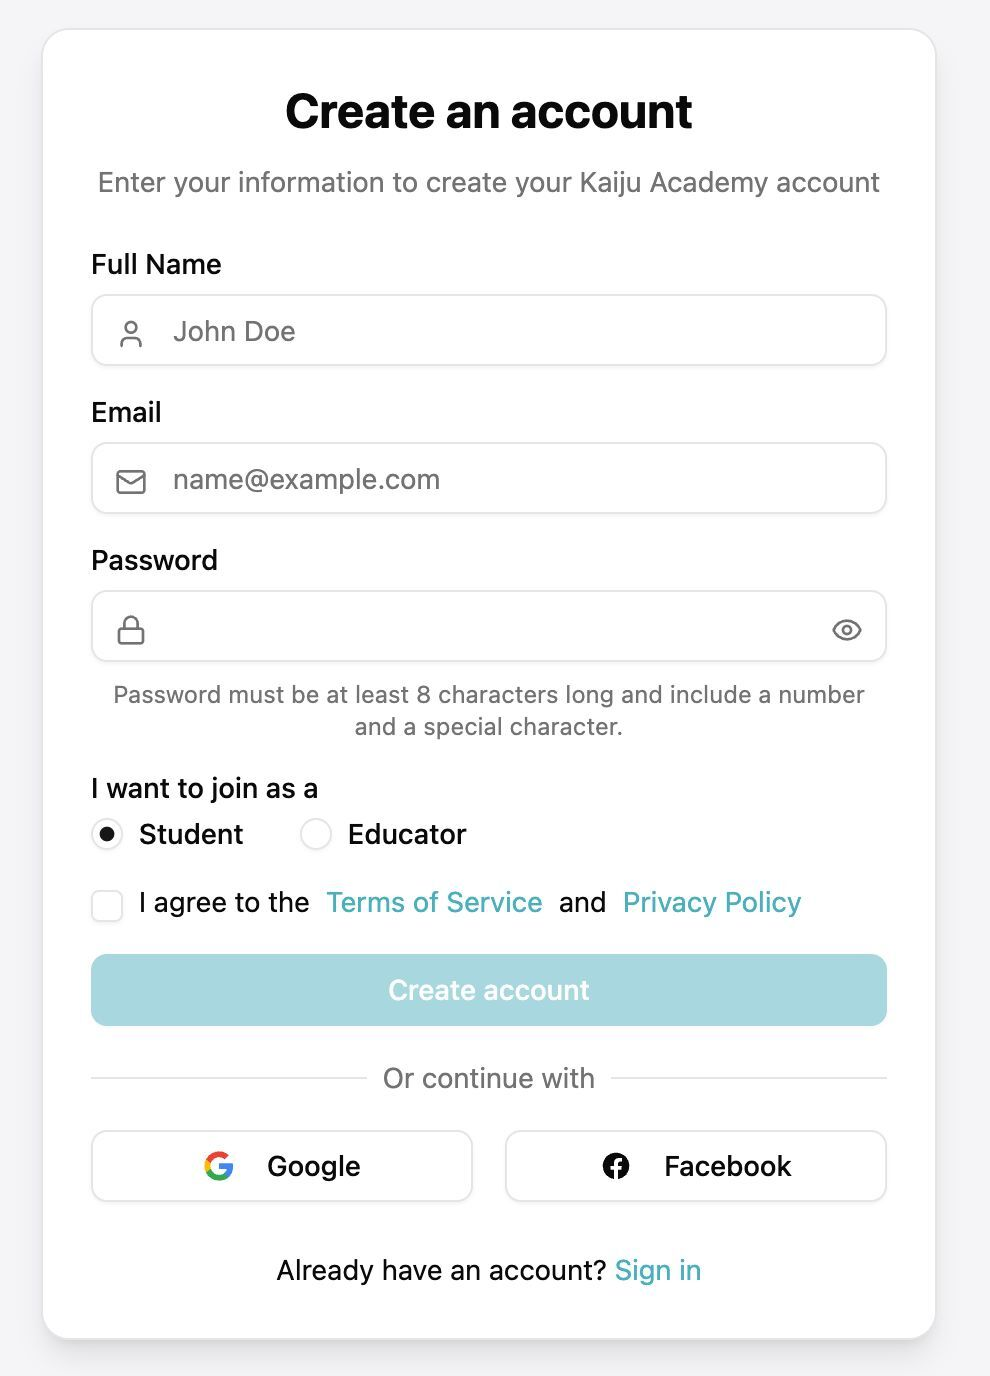
\includegraphics[width=0.5\textwidth]{SignUp.jpg}
    \caption{Sign Up Screen}
\end{figure}

\subsection{Login}
\begin{enumerate}[leftmargin=*]
    \item Click \textbf{Sign In}.
    \item Enter your email and password.
    \item If MFA is enabled, enter your authentication code.
    \item You can also sign in with Google or Facebook.
    \item Upon successful login, you will be redirected to your dashboard.
\end{enumerate}
\begin{figure}[H]
    \centering
    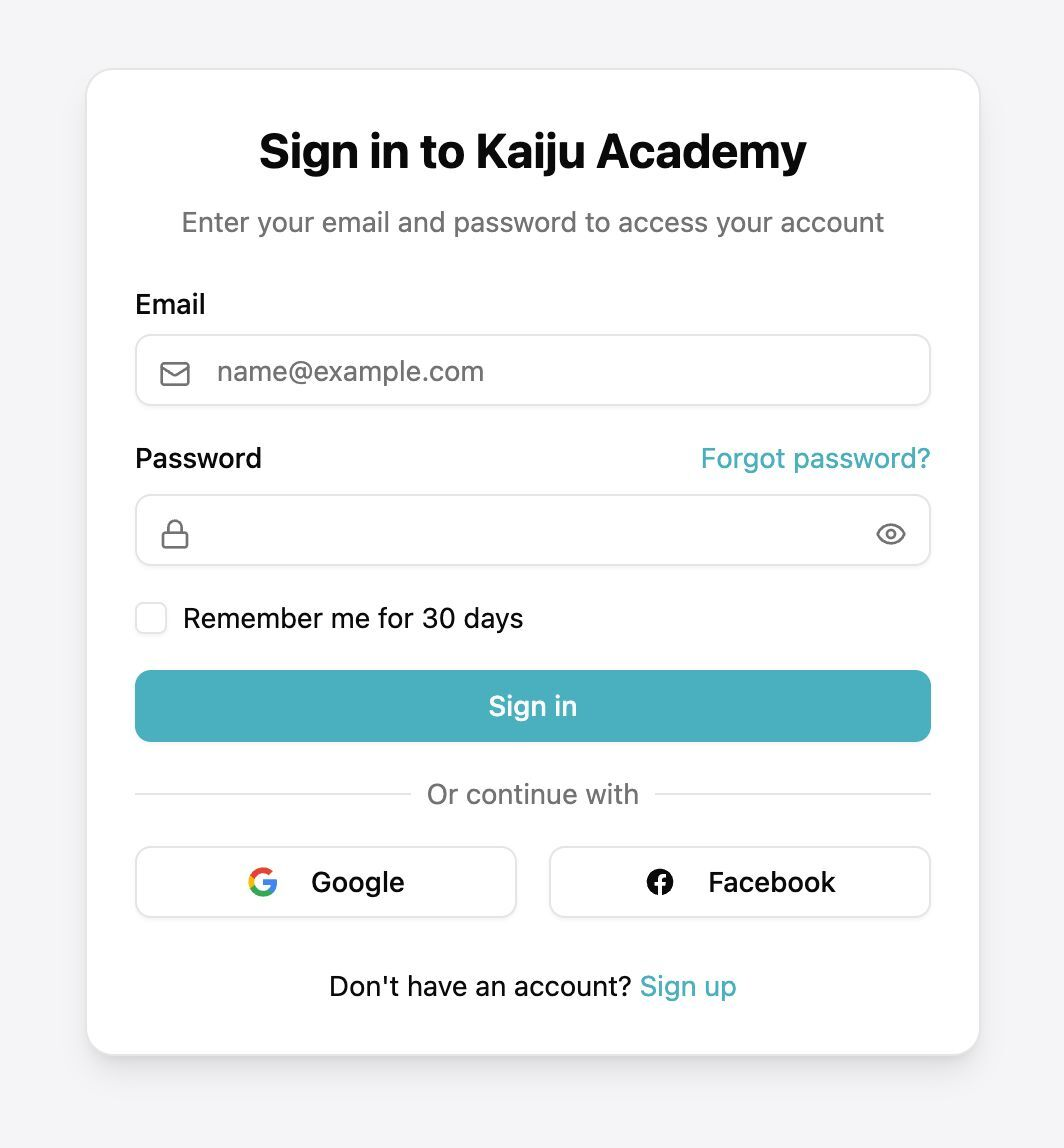
\includegraphics[width=0.5\textwidth]{SignIn.jpg}
    \caption{Sign In Screen}
\end{figure}

\section{Credits and Licence Key System}

\subsection{Overview}
Kaiju Academy uses a credit-based system to unlock paid courses. Credits can be obtained in two ways:
\begin{itemize}[leftmargin=*]
    \item \textbf{Purchase credits}: Pay with a credit card via a secure payment gateway.
    \item \textbf{Redeem a licence key}: Enter a valid licence key purchased from authorized distributors to top up your credits.
\end{itemize}

\subsection{Buying or Redeeming Credits}
\begin{enumerate}[leftmargin=*]
    \item Go to \textbf{Buy Credits} in your dashboard or profile.
    \item Select a credit package.
    \item Choose your payment method:
    \begin{itemize}
        \item To buy with a card, proceed to the payment gateway and complete your purchase.
        \item To redeem a licence key, click \textbf{Redeem Key}, then enter your licence key and submit.
    \end{itemize}
    \item After a successful transaction or key redemption, your credit balance will be updated.
\end{enumerate}
\textbf{Security Note:} All payment processing is handled by a PCI-compliant gateway. No sensitive payment data is stored on Kaiju Academy servers. Licence keys are securely generated and stored; do not share your key with others.

\subsection{Enrolling in Paid Courses}
\begin{enumerate}[leftmargin=*]
    \item Browse available courses.
    \item Click \textbf{Enroll} on a course (requires enough credits).
    \item Confirm enrollment; credits will be deducted from your account.
    \item If you don’t have enough credits, you will be prompted to buy or redeem more.
\end{enumerate}

\section{User Roles and Dashboard Overview}

\subsection{Students}
\begin{itemize}[leftmargin=*]
    \item View enrolled courses, progress, and recommended courses.
    \item Access interactive coding assignments and submit solutions.
    \item Purchase or redeem credits to unlock new courses.
\end{itemize}
\begin{figure}[H]
    \centering
    
\includegraphics[width=0.95\textwidth]{myCourse.jpg}
    \caption{Student's My Courses View}
\end{figure}

\subsection{Educators}
\begin{itemize}[leftmargin=*]
    \item Create, update, or delete courses and modules.
    \item Upload materials (videos, PDFs, problems).
    \item View and grade student submissions.
    \item Track course statistics and student progress.
\end{itemize}
\begin{figure}[H]
    \centering
    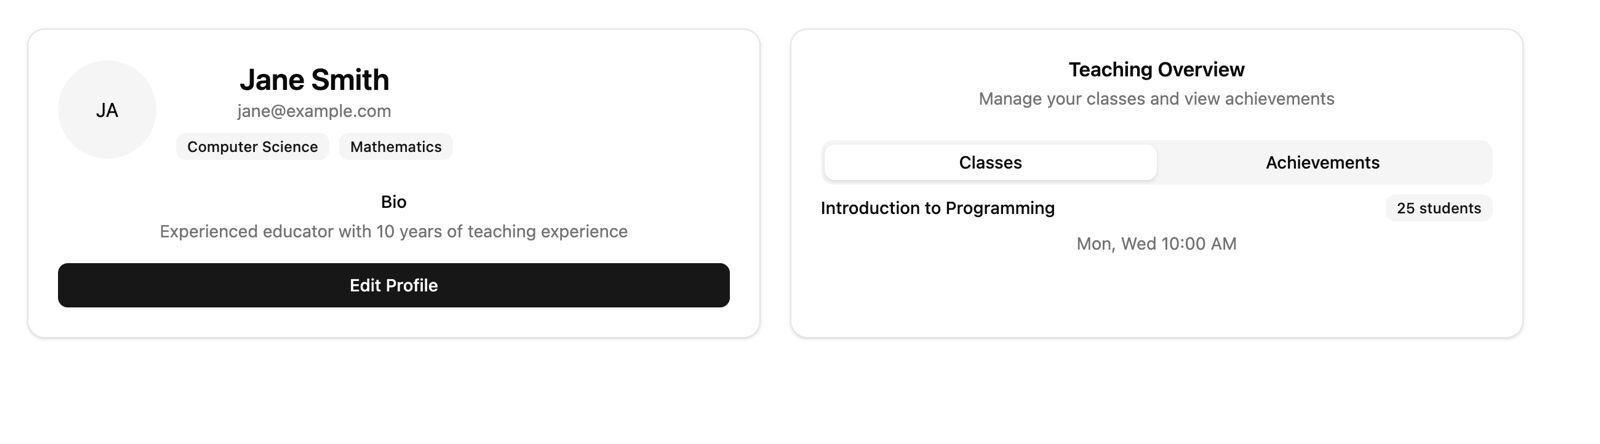
\includegraphics[width=0.95\textwidth]{TeacherProfile.jpg}
    \caption{Educator Profile and Teaching Overview}
\end{figure}

\subsection{Navigating the Dashboard}
\begin{itemize}[leftmargin=*]
    \item Use the navigation bar to access \texttt{Courses}, \texttt{Profile}, \texttt{Credit Purchase}, and \texttt{Support}.
\end{itemize}
\begin{figure}[H]
    \centering
    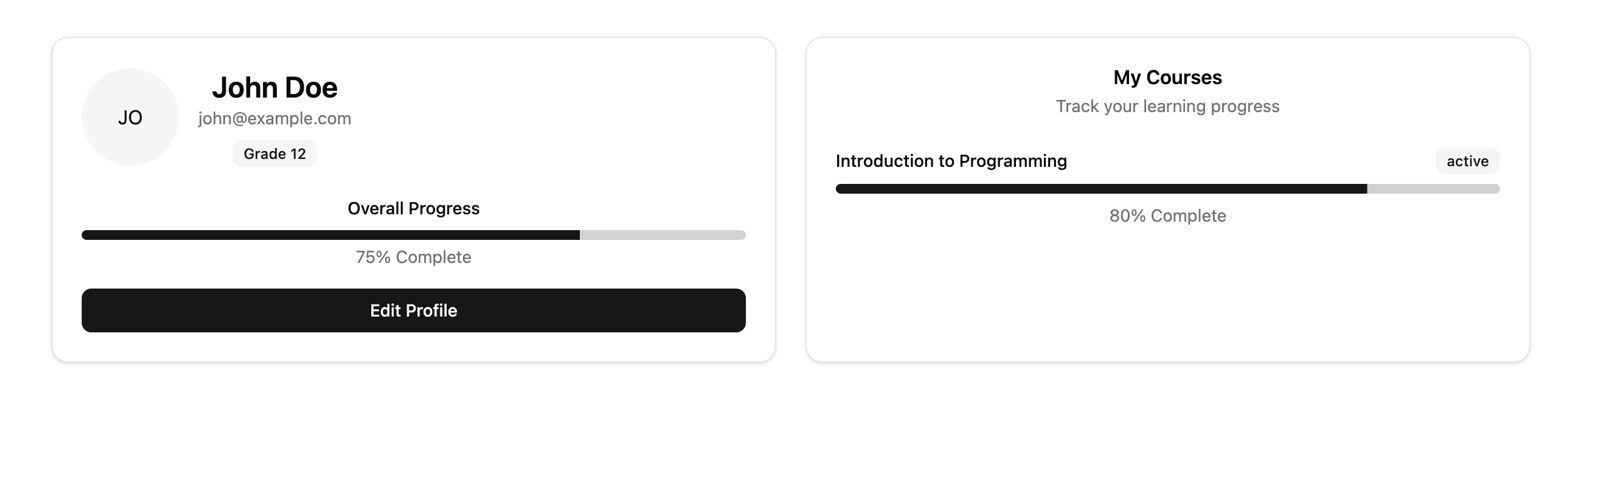
\includegraphics[width=0.85\textwidth]{StudentProfile.jpg}
    \caption{User Dashboard and Progress Tracking}
\end{figure}

\section{Courses}

\subsection{Browsing and Enrolling}
\begin{enumerate}[leftmargin=*]
    \item Click on \textbf{Courses}.
    \item Browse or search for available courses.
    \item To enroll, click \textbf{Enroll} (requires sufficient credits for paid courses).
    \item Confirm enrollment; the course will appear in your dashboard.
\end{enumerate}
\begin{figure}[H]
    \centering
    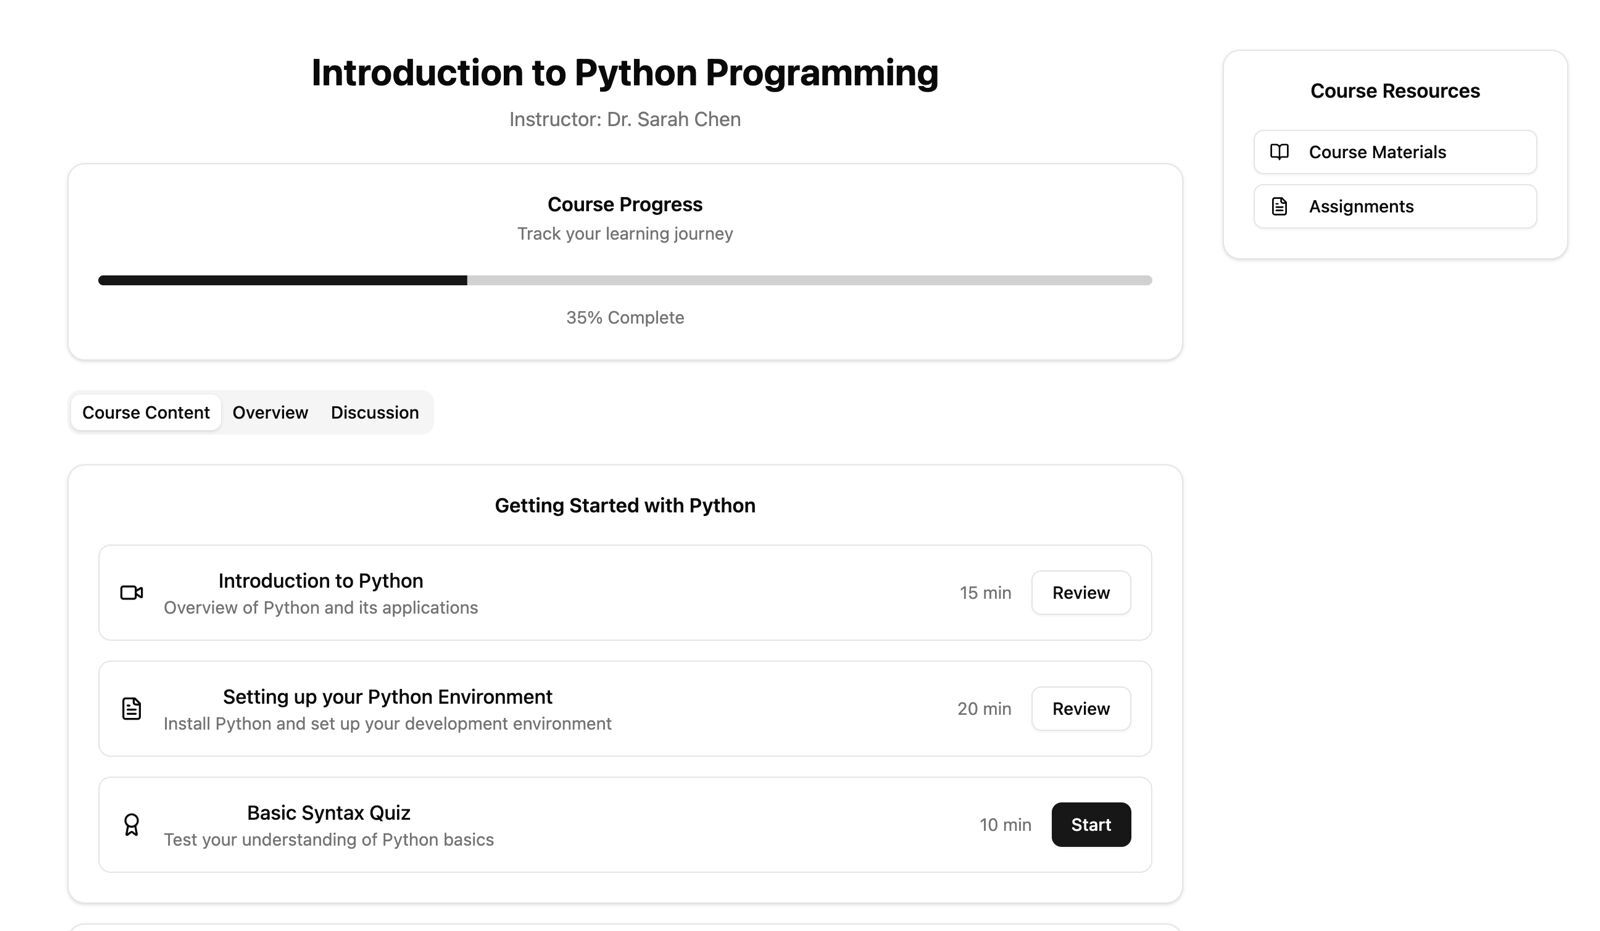
\includegraphics[width=0.95\textwidth]{CourseDetail.jpg}
    \caption{Course Detail and Progress}
\end{figure}

\subsection{Course Content}
\begin{itemize}[leftmargin=*]
    \item Courses contain modules with lectures, readings, and assignments.
    \item Completed modules are tracked in your profile.
\end{itemize}

\section{Interactive Code Assessment}

\begin{enumerate}[leftmargin=*]
    \item Open a course and select a coding assignment.
    \item Write or edit your code in the provided editor.
    \item Click \textbf{Run} to execute and see results/output.
    \item Click \textbf{Submit} to grade your solution.
    \item View feedback and results.
\end{enumerate}
\begin{figure}[H]
    \centering
    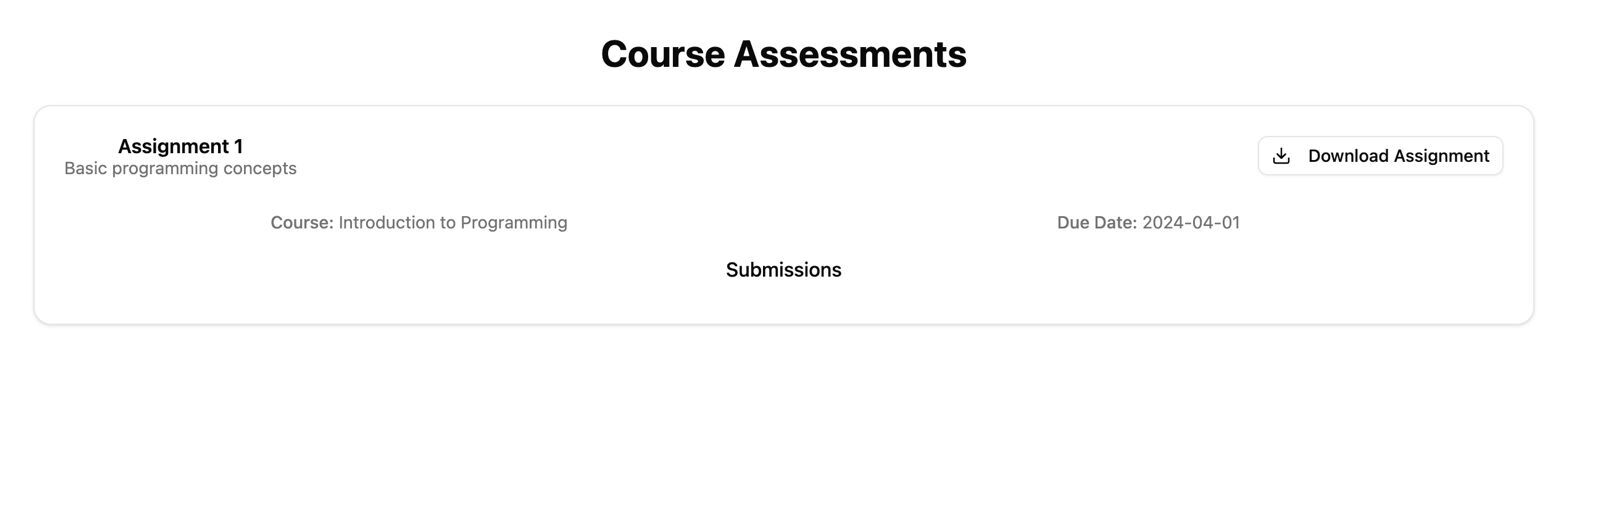
\includegraphics[width=0.95\textwidth]{StudentAssessment.jpg}
    \caption{Student Assessment Interface}
\end{figure}

\section{Educator Features}

\subsection{Course Management}
\begin{figure}[H]
    \centering
    
\includegraphics[width=0.95\textwidth]{TeacherManageCourse.jpg}
    \caption{Educator Course Management}
\end{figure}
\begin{enumerate}[leftmargin=*]
    \item Access course management from your educator dashboard.
    \item Create new courses or edit existing ones.
    \item Add modules, assignments, and update course descriptions.
\end{enumerate}

\subsection{Edit Course}
\begin{figure}[H]
    \centering
    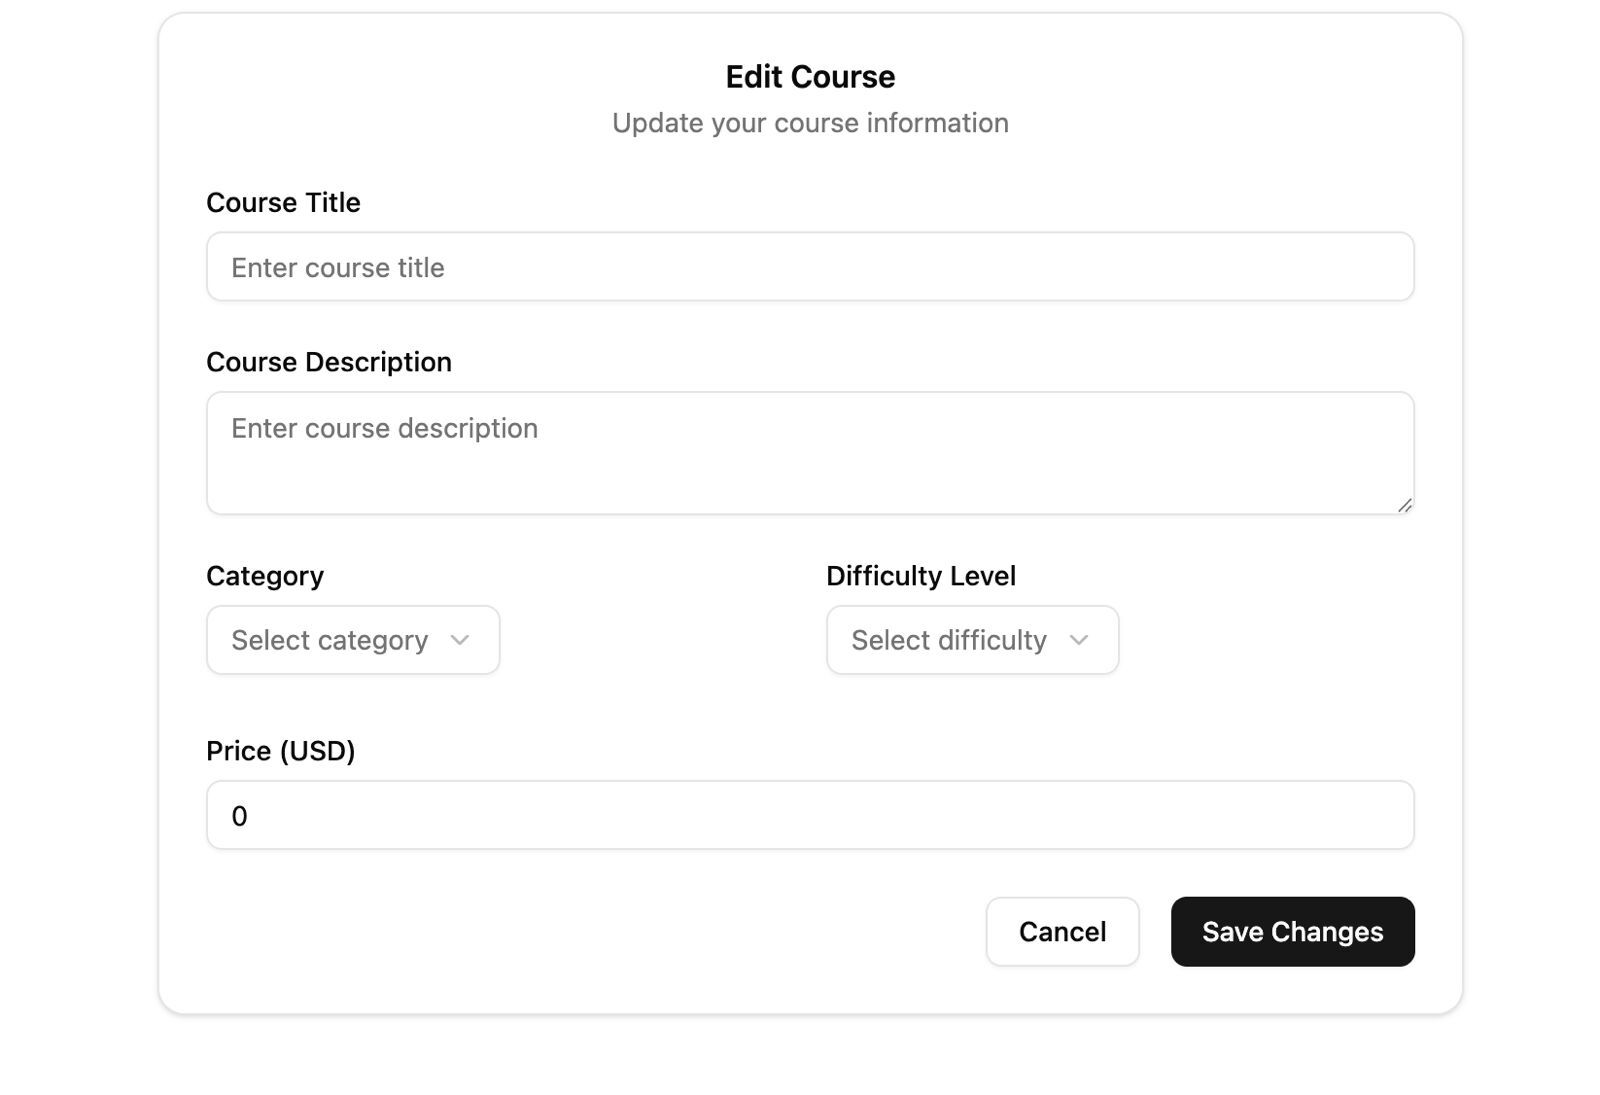
\includegraphics[width=0.7\textwidth]{TeacherEditCourse.jpg}
    \caption{Edit Course Screen}
\end{figure}

\subsection{Assessment Management}
\begin{figure}[H]
    \centering
    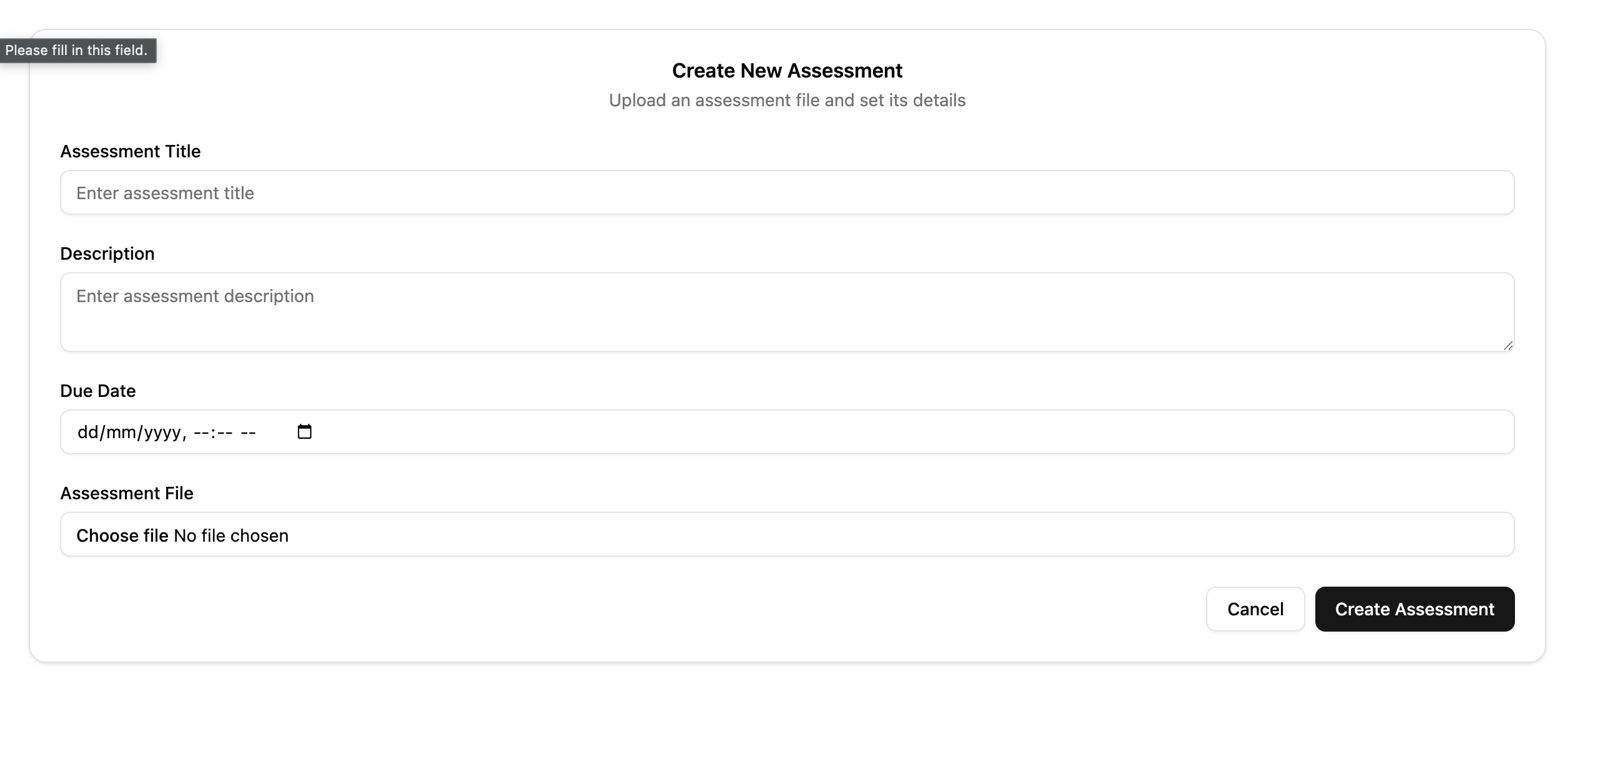
\includegraphics[width=0.95\textwidth]{TeacherCreateAssessment.jpg}
    \caption{Create New Assessment}
\end{figure}
\begin{figure}[H]
    \centering
    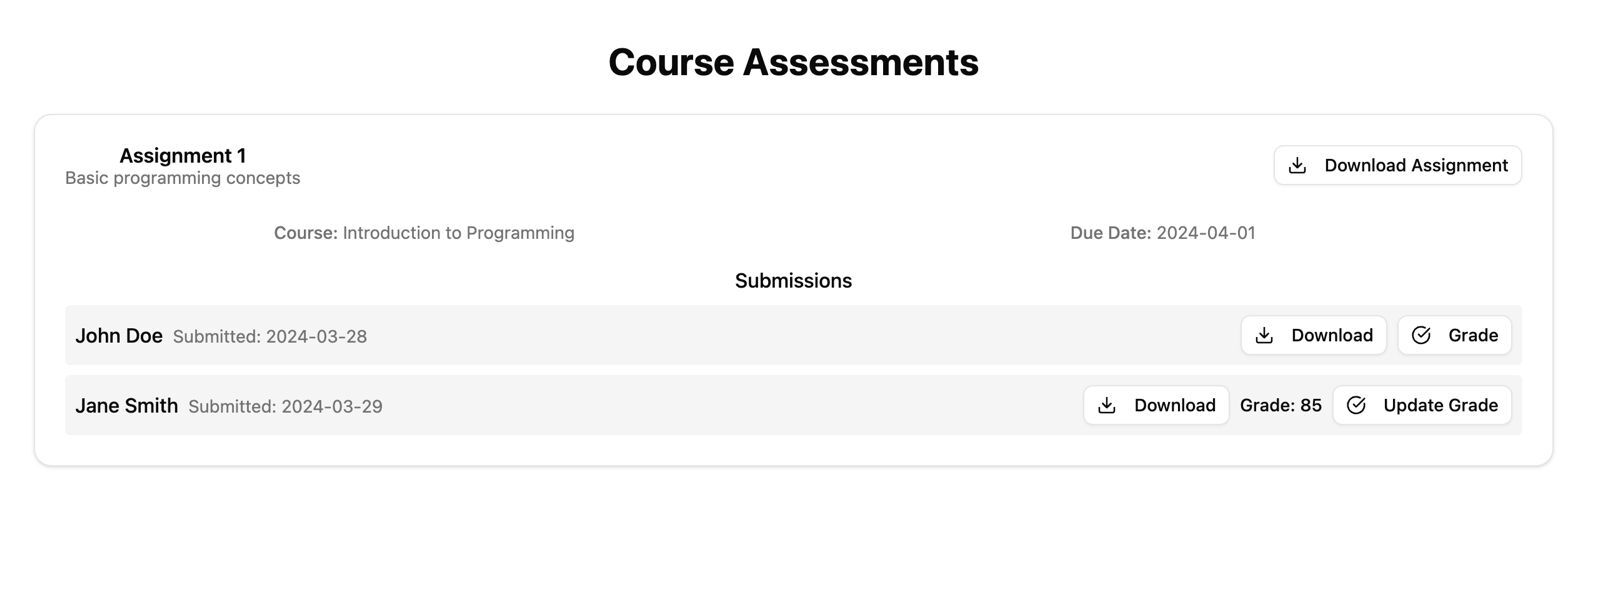
\includegraphics[width=0.95\textwidth]{TeacherAssessment.jpg}
    \caption{Assessment Grading and Submissions}
\end{figure}

\section{Profile and Progress Tracking}
\begin{itemize}[leftmargin=*]
    \item Access your profile to view enrolled and recommended courses.
    \item Track progress (completion percentage, badges, achievements).
    \item Update your personal details or change password.
\end{itemize}

\section{Error Handling and Support}
\begin{itemize}[leftmargin=*]
    \item Common error messages (e.g., invalid login, insufficient credits) are displayed on screen.
    \item For technical issues, contact support at \href{mailto:support@kaijuacademy.example.com}{support@kaijuacademy.example.com}.
\end{itemize}

\section{Frequently Asked Questions (FAQ)}

\begin{itemize}[leftmargin=*]
    \item \textbf{Q: I forgot my password. What should I do?}
    \begin{itemize}
        \item Click \textbf{Forgot Password} on the login page and follow the instructions.
    \end{itemize}
    \item \textbf{Q: How do I get more credits?}
    \begin{itemize}
        \item Use the \textbf{Buy Credits} page in your dashboard.
    \end{itemize}
    \item \textbf{Q: Who do I contact for billing issues?}
    \begin{itemize}
        \item Email: \href{mailto:support@kaijuacademy.example.com}{support@kaijuacademy.example.com}
    \end{itemize}
    \item \textbf{Q: My licence key is not working. What should I do?}
    \begin{itemize}
        \item Double-check your key for typos. If it still does not work, contact support.
    \end{itemize}
\end{itemize}

\section{Contact and Support}
\begin{itemize}[leftmargin=*]
    \item For technical support or feedback, contact: \href{mailto:support@kaijuacademy.example.com}{support@kaijuacademy.example.com}
    \item For course content questions, contact your educator via the course page.
\end{itemize}

\section{Acknowledgments}
This document was prepared with the assistance of AI tools (e.g., ChatGPT 4.1) for drafting and review.

\end{document}